\documentclass[12pt,a4paper]{article}
\usepackage{tikz}
\usetikzlibrary{arrows}
\usepackage{latexsym}
\usepackage{tech}
\usepackage{scalalistings}

\newtheorem{lemma}{Lemma}

\def\s#1{$_{#1}$}

\title{Understanding synchronisation}
\author{Jonathan Lawrence and Gavin Lowe}

\begin{document}
\maketitle

Idea of synchronisation.  Consider synchronisation of just two threads, for
ease of exposition.  Each passes in some parameters, and receives back a
result.  
\begin{scala}
  def op£\s1£(x£\s1£: A£\s1£): B£\s1£
  def op£\s2£(x£\s2£: A£\s2£): B£\s2£
\end{scala}
In addition, the synchronisation object might have some state $state: S$.
Each result may depend on the two parameters |x|$_1$ and |x|$_2$ and the
current state.  In addition, the state may be updated.  This all appears to
happen atomically at some point within the duration of both operation
invocations (which implies that the invocation must overlap.

The synchronisation can be specified by a sequential specification object with
the following signature.
%
\begin{scala}
object Spec{
  private state: S
  def sync(x£\s1£: A£\s1£, x£\s2£: A£\s2£): (B£\s1£, B£\s2£)
}
\end{scala}
%
The idea is that if two invocations |op|\s1|(x|\s1|)| and |op|\s2|(x|\s2|)|
synchronise, then the results |y|\s1 and |y|\s2 of the invocations are such
that |sync(x|\s1|, x|\s2|)| could return the pair |(y|\s1|, y|\s2|)|, and the
|state| is updated in the same way.  A typical definition of |sync| might take
the form
\begin{scala}
  def sync(x£\s1£: A£\s1£, x£\s2£: A£\s2£): (B£\s1£, B£\s2£) = {
    require(guard(x£\s1£, x£\s2£, state))
    val res£\s1£ = f£\s1£(x£\s1£, x£\s2£, state); val res£\s2£ = f£\s2£(x£\s1£, x£\s2£, state)
    state = update(x£\s1£, x£\s2£, state)
    (res£\s1£, res£\s2£)
  }
\end{scala}

For example, consider a synchronous channel with signature
\begin{scala}
class SyncChan{
  def send(x: A): Unit
  def receive(u: Unit): A
}
\end{scala}
%
(Note that we model the |receive| operation as taking a parameter of type
|Unit|, which is the singleton type containing just the unit value, denoted
``|()|''.) 
%
This can be specified using a sequential specification object with empty
state, and with 
\begin{scala}
  def sync(x: A, u: Unit): (Unit, A) = ((), x)
\end{scala}

Another example: a filtering channel.
\begin{scala}
class FilterChan{
  def send(x: A): Unit
  def receive(p: A => Boolean): A
}
\end{scala}
Can be specified with
\begin{scala}
  def sync(x: A, p: A => Boolean): (Unit, A) = { require(p(x)); ((), x) }
\end{scala}

As an example illustrating the use of state in the synchronisation object,
suppose that the synchronisation object maintains a sequence counter, and both
invocations receive the value of this counter.  That is, the channel has
signature 
\begin{scala}
class SyncChanSeqCounter{
  def send(x: A): Int
  def receive(u: Unit): (A, Int)
}
\end{scala}
%
This can be specified using the following specification object.
%
\begin{scala}
object SyncChanSeqCounterSpec{
  private var counter = 0
  def sync(x: A, u: Unit): (Int, (A, Int)) = {
    counter += 1; (counter, (x, counter))
  }
}
\end{scala}

%%%%%%%%%%%%%%%%%%%%%%%%%%%%%%%%%%%%%%%%%%%%%%%%%%%%%%%

\subsection*{Formal definition}

State definition of linearisability here. 

Following definition of linearisation.  History of synchronisation object,
containing call and return events, with matching invocation indices,
e.g. $call.\sm{op}_1^{i_1}(x_1)$ and $return.\sm{op}_1^{i_1}: y_1$; indiced
otherwise distinct.  History of sequential specification object, with events
representing (atomic) invocations of sync, labelled with a pair of invocation
indices, e.g.~$\sm{sync}^{i_1, i_2}(x_1, x_2): (y_1, y_2)$.  No invocation
index is repeated in the history.  Define ``legal'' in the normal way.  Define
interleaving of concurrent and sequential history: each |sync| has to be
between the corresponding $call$ and $return$ for each of the two invocations.

Maybe call this \emph{synchronisation linearisation}. 


%%%%%%%%%%%%%%%%%%%%%%%%%%%%%%%%%%%%%%%%%%%%%%%%%%%%%%%

\subsection*{Relating synchronisation and linearisation}

Need to allow one of the operations on the concurrent object to linearise
\emph{two} operations on the linearisability specification.  Formal definition
of this.  Linearisability specification object has signature
%
\begin{scala}
object LinSpec{
  def seqOp£\s1£(x£\s1£: A£\s1£): Unit
  def £$\overline{\sm{seqOp}}_1$£(): B£\s1£
  def seqOp£\s2£(x£\s2£: A£\s2£): B£\s2£
}
\end{scala}
%
The idea is that the operation |op|\s1 on the concurrent object will be
linearised by the composition of the two operations |seqOp|\s1 and
$\overline{\sm{seqOp}}_1$.  What this means formally: in the interleaved
history, the events of the two sequential operations are between the
corresponding $call$ and $return$ events, in that order. 

Formal definition. 

Given a synchonisation specification object |SyncSpec|, we build a corresponding linearisation specification object.
\begin{scala}
trait LinState
case class Zero extends LinState
case class One(x£\s1£: A£\s1£) extends LinState
case class Two(y£\s1£: B£\s1£) extends LinState

object LinSpec{
  private var linState: LinState = Zero
  def seqOp£\s1£(x£\s1£: A£\s1£): Unit = {
    require(linState.isInstanceOf[Zero]); linState = One(x£\s1£)
  }
  def seqOp£\s2£(x£\s2£: A£\s2£): B£\s2£ = {
    require(linState.isInstanceOf[One]); val One(x£\s1£) = linState
    val (y£\s1£, y£\s2£) = SyncSpec.sync(x£\s1£, x£\s2£); linState = Two(y£\s1£); y£\s2£
  }
  def £$\overline{\sm{seqOp}}_1$£(): B£\s1£ = {
    require(linState.isInstanceOf[Two]); val Two(y£\s1£) = linState; linState = Zero; y£\s1£
  }
}
\end{scala}
%
The behaviour of the linearisation specification object is captured by the
following automaton.
%
\begin{center}
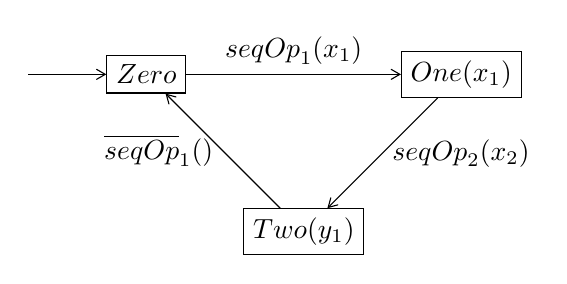
\begin{tikzpicture}[>= angle 60]
\draw (0,0) node[draw] (zero) {$\sm{Zero}$};
\draw[->] (zero) ++ (-1.5, 0) -- (zero);
%
\draw (4,0) node[draw] (one) {$\sm{One}(\sm{x}_1)$};
\draw[->] (zero)  -- node[above] {$\sm{seqOp}_1(\sm{x}_1)$} (one); 
%
\draw (2, -2) node[draw] (two) {$\sm{Two}(\sm{y}_1)$};
\draw[->] (one)  -- node[right] {$\sm{seqOp}_2(\sm{x}_2)$} (two); 
\draw[->] (two) -- node[left] {$\overline{\sm{seqOp}}_1()$} (zero);
\end{tikzpicture}
\end{center}
%
The definition of the linearisation specification object forces the operations
to take place in the order described by the automaton.  The |seqOp|\s2
operation calls the |sync| method on |SyncSpec|, to calculate the return
values and to update the state: in effect, the synchronisation happens at this
point. 

\begin{lemma}
If the concurrent object is linearisable with respect to |LinSpec|, then its
synchronisations satisfy |SyncSpec|.
\end{lemma}
%
\begin{proof}
Idea: given a linearisation history, we can take the synchronisation point to
be the linearisation point of $\sm{seqOp}_2$.
\end{proof}

\begin{lemma}
If the concurrent object's synchronisations satisfy |SyncSpec|, then it is
linearisable with respect to |LinSpec|.
\end{lemma}
%
\begin{proof}
Idea: given a synchronisation history, we can replace the synchronisation
point by the linearisation points of the three operations of |LinSpec| to
create the linearisation history. 
\end{proof}



%%%%%%%%%%%%%%%%%%%%%%%%%%%%%%%%%%%%%%%%%%%%%%%%%%%%%%%

\subsection*{Testing algorithms}

Overview of linearisability testing framework. 

Note, assumes deterministic specification object. 

\subsubsection*{Case with state}

Suppose the specification object has non-trivial state. 

Could adapt linearisability testing framework following previous result.  Need
to allow an operation to be linearised by two operations.

I think it will be more efficient to give a more direct implementation.
Define a configuration to be: (1)~a point in the log reached so far; (2)~the
set of pending operation invocations that have not synchronised; (3)~the set
of pending operation invocations that have synchronised (but not returned);
and (4)~the state of the sequential synchronisation object.  In any
configuration, can: synchronise a pair of pending operations (and update the
synchronisation object); advance in the log if the next event is a return that
is not pending; or advance in the log if the next event is a call.  Then
perform DFS.

Partial order reduction: a synchronisation point must follow either the
call of one of the concurrent operations, or another synchronisation
point.  Any synchronisation history can be transformed into this form, by
moving synchronisation points earlier, but not before any of the corresponding
call events, and preserving the order of synchronisations.  

Alternatively, a synchronisation point must precede either the return of one
of the concurrent operations, or another synchronisation point.  This is more
like the JIT technique in the linearisability testing paper.  This means that
before advancing in the log to the return of an invocation that has not
synchronised, we synchronise some invocations, ending with the one in
question.  And we only synchronise in these circumstances. 

%%%%%

\subsubsection*{Complexity}

Consider the problem of testing whether a given concurrent history has
synchronisations consistent with a given sequential specification object. 

We make use of a result from~\cite{???} concerning the complexity of the
corresponding problem for linearizability.  Let |Variable| be a
linearizability specification object corresponding to a variable with |get|
and |set| operations.  Then the problem of deciding whether a given concurrent
history is linearisable with respect to |Varaiable| is NP-complete.

Let |ConcVariable| be a concurrent object that represents a variable.  

We consider concurrent synchronisation histories on an object with the
following signature.   
\begin{scala}
object VariableSync{
  def op£\s1£(op: String, x: Int): Int
  def op£\s2£(u: Unit): Unit
} 
\end{scala}
%
The intention is that |op|\s1|("get", x)| acts like |get(x)|, and
|op|\s1|("set", x)| acts like |set(x)| (but returns -1).  The |op|\s2
invocations do nothing except synchronise.  This can be captured formally by
the following synchronisation specification object.

\begin{scala}
object VariableSyncSpec{
  private var state = 0
  def sync((op, x): (String, Int), u: Unit): (Int, Unit) = 
    if(op == "get") (state, ()) else{ state = x; (-1, ()) }
}
\end{scala}


Let |ConcVariable| be a concurrent object that represents a variable.  Given a
concurrent history~$h$ of |ConcVariable|, we build a concurrent history~$h'$
of |VaraibleSync| as follows.  We replace every call or return of |get(x)| by
(respectively) a call or return of |op|\s1|("get", x)|; and we do similarly
with |set|s.  If there are $k$ calls of |get| or |set| in total, we prepend
$k$ calls of |op|\s2, and append $k$ corresponding returns (in any order).
Then it is clear that $h$ is linearisable with respect to |Variable| if and
only if $h'$ is linearisable with respect to |VariableSyncSpec|.

%%%%%

\subsubsection*{Stateless case}

In the stateless case, a completely different algorithm is possible.  Define
two invocations to be compatible if they could be synchronised, i.e.~they
overlap and the return values agree with those for the specification object.
For $n$ invocations of each operation (so a history of length~$4n$), this can
be calculated in $O(n^2)$.  Then find if there is a total matching in the
corresponding bipartite graph, using the Ford-Fulkerson method, which is
$O(n^2)$.

%%%%%%%%%%%%%%%%%%%%%%%%%%%%%%%%%%%%%%%%%%%%%%%%%%%%%%%

\subsection*{Variations}

We've implicitly assumed that the operations |op|\s1 and |op|\s2 are
distinct.  I don't think there's any need for this.  Example: exchanger.  

Most definitions and results go through to the case of $k > 2$ invocations
synchronising.  Examples: ABC problem; barrier synchronisation.  To capture
the relationship with linearisation, we require $k-1$ operations to be
linearised by two operations of the specification object.  Maybe give
automaton for $k = 4$.  

I suspect the complexity in the stateless case is NP-complete for $k > 2$.
Finding a maximum matching in a 3-partite hypergraph is NP-complete; see
\verb|https://en.wikipedia.org/wiki/3-dimensional_matching|.

%% Complexity result in the stateless case.  Build a weighted graph with nodes as
%% follows. 
%% %
%% \begin{itemize}
%% \item For each tuple $(i_1, \ldots, i_k)$ such that $\sm{op}_1^{i_1}, \ldots
%%   \sm{op}_k^{i_k}$ that could be synchronised (i.e.~they all overlap and the
%%   return values agree with specification object), we include a node $(i_1,
%%   \ldots, i_k)$; we call these \emph{tuple nodes}.  If there are $n$
%%   invocations of each operation, these nodes can be constructed in time
%%   $O(n^k)$. 

%% \item For each~$j$ and invocation $\sm{op}_j^{i}$, we include a node $(j, i)$.

%% \item We include source and target nodes~$s$ and~$t$.
%% \end{itemize}
%% %
%% We include edges as follows.
%% %
%% \begin{itemize}
%% \item For each $\sm{op}_j^{i}$, we include an edge with capacity~1 from~$s$
%%   to~$(j,i)$; and an edge with capacity~1 to each corresponding tuple node,
%%   i.e.~those tuple nodes that have index~$i$ in position~$j$. 

%% \item For each tuple node, we include an edge with capacity~$k$ to~$t$.
%% \end{itemize}
%% %
%% If the history is synchronisation-linearisable, then the graph has a flow
%% of~$n \times k$, with a

Some synchronisation objects allow different modes of synchronisation.  For
example, consider a synchronous channel with timeouts: each invocation might
synchronise with another invocation, or might timeout without
synchronisation.  Such a channel might have a signature as follows.
%
\begin{scala}
class TimeoutChannel{
  def send(x: A): Boolean
  def receive(u: Unit): Option[A]
}
\end{scala}
%
The |send| operation returns a boolean to indicate whether the send was
successful, i.e.~whether it synchronised.  The |receive| operation can return
a value |Some(x)| to indicate that it synchronised and received~|x|, or can
return the value |None| to indicate that it failed to synchronise (the type
|Some[A]| contains the union of such values).  The possible synchronisations
can be captured by the following specification object.
\begin{scala}
object TimeoutSpec{
  def sync£$_{s,r}$£(x: A, u: Unit): (Boolean, Option[A]) = (true, Some(x))
  def sync£$_s$£(x: A): Boolean = false
  def sync£$_r$£(u: Unit): Option[A] = None
}
\end{scala}
%
The operation $\sm{sync}_{s,r}$ corresponds to where a |send| and |receive|
synchronise, as previously.  The operations $\sm{sync}_s$ and $\sm{sync}_r$
correspond, respectively, to where a |send| or |receive| fails to
synchronise.  

More generally, the specification object can have any number of operations of
the form
%
\begin{scala}
  def sync£$_{j_1, \ldots, j_m}$£(x£\s1£: A£\s1£, £\ldots£, x£\s m£: A£\s m£): (B£\s1£, £\ldots£, B£\s m£)
\end{scala}
%
This corresponds to the case of a synchronisation between the $m$~invocations
$\sm{op}_{j_1}(\sm x_1), \ldots, \sm{op}_{j_m}(\sm x_m)$.  The formal
definition is an obvious adaptation of the previous version: in the
interleaved history, between the call and return of each $\sm{op}_j(\sm x):
\sm y$, there must be a corresponding $\sm{sync}_{j_1, \ldots, j_m}(\sm x_1,
\ldots \sm x_m): (\sm y_1, \ldots, \sm y_m)$ event, i.e.~for some~$i$,\, $j =
j_i$,\, $\sm x = \sm x_i$, and $\sm y = \sm y_i$.


%%%%%%%%%%%%%%%%%%%%%%%%%%%%%%%%%%%%%%%%%%%%%%%%%%%%%%%

\subsection*{Misc}

Is the definition compositional? 

\end{document}
